% Chapter Template

\chapter{Problem Solution} % Main chapter title

\label{Chapter6} % Change X to a consecutive number; for referencing this chapter elsewhere, use \ref{ChapterX}

\lhead{Chapter 6. \emph{Problem Solution}} % Change X to a consecutive
% number; this is for the header on each page - perhaps a shortened title

%----------------------------------------------------------------------------------------
%	SECTION 1
%----------------------------------------------------------------------------------------
\pagestyle{empty} 
\section{Integrate Henshin with DPF}

DPF is a a framework where it is possible to create an arbitrary levels of
meta-models, and that gives the users the freedom to define a well formed domain
specific modeling language and to define constraints for each specification at
each level of meta-modeling. The framework provides the possibility to define
specifications that specify underlying specifications. Where each specification
$\spec{S}$\textsubscript{n+1} defines the abstract syntax for a specification
$\spec{S}$\textsubscript{n}. For DPF to be a framework that follows the visions
of model driven engineering it needs to have support for automation of
specifications over different levels of abstraction. It already has support for
some cases of model transformations. There is one natural model transformation
for DPF when specifying a new specification. A new specification will always be
specified by a modeling language that corresponds to a specification
$\spec{S}$\textsubscript{n+1}. These specification may either be a user created
specification or the default specification provided by the framework, that
conforms to it self. The creation of a new specification can be viewed as the
first support for automation over levels of abstraction for models that the
Diagram Predicate Framework povides. In 2012 Anders Sandven published his
master thesis\cite{Sandven_thesis}, where he implemented support for generating
source code with the DPF Editor. DPF does not provide support for applying an
exogenous model transformation to a specification described in one domain
specific modeling language to a model expressed in another domain specific
modeling language. To achieve this we want to integrate Henshin transformation
language\cite{Arendt2010} to the framework.

\begin{figure}[H]
	\centering
	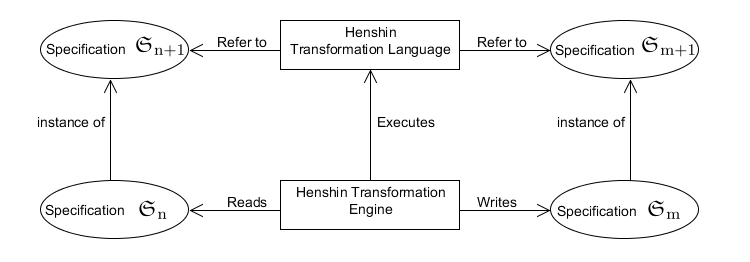
\includegraphics[scale=0.7]{./Figures/TransformationSolutionBasic.png}
	\caption[Integrating Henshin with DPF]
	{Using Henshin transformation language to translate a specification
	$\spec{S}$\textsubscript{n}.}
	\label{fig:Simple_Solution}
\end{figure}

Figure~\ref{fig:Simple_Solution} explains how we want to integrate the Henshin
model transformation language with the Diagram Predicate Framework. Henshin
provides a transformation language and a transformation engine. We
use the Henshin transformation engine to read an instance specification
$\spec{S}$\textsubscript{n} and write an instance specification
$\spec{S}$\textsubscript{m}. To achieve this the transformation engine executes
a set of transformation rules written in the Henshin Transformation Language.
These transformation rules refers to the abstract syntax for the
specification $\spec{S}$\textsubscript{n+1} and specification
$\spec{S}$\textsubscript{m+1} that the source and target model are typed over.

The problem with integrating Henshin with DPF is that Henshin is implemented by
EMF, and therefore utilize OMG's MOF. The Henshin model transformation
language create the transformation rules based on models that are created
accordingly to the four layer meta-modeling provided by MOF. The
specification implementation for a DPF model is created as an EMF meta-model 
and utilize the EMF Genmodel to provide code generation. DPF provides
initialisation of a potential endless hierarchy of meta-models, and therefore
does not match the steps MOF provides to create abstract syntax for a domain
specific language. It is however important to separate the implementation of a
specification and the creation of a new specification. Because DPF utilize EMF
to some extent. Each model created in DPF represents the lowest layer of
meta-modeling in MOF, regardless of the level of abstraction the model
represents. However what makes DPF unique compared to EMF is that a DPF model us
an instance model of both an Ecore meta-model and another DPF model. This means
that a DPF models concrete syntax is typed by the abstract syntax of another DPF
model. While all modeling elements from these models conforms to one common
meta-model. In DPF we can create an arbitrary level of meta-models and therefore
each domain specific modeling language defined in the framework can have
different layers of specification models. The Henshin environment has strict
guidelines on how models are imported and used. These models are required to be
created accordingly to and typed by the Ecore model provided by EMF. Henshin
can then utilize these models to create a graph pattern that structure both the
LHS and the RHS graph of a transformation rule.

\begin{figure}[H]
	\centering
	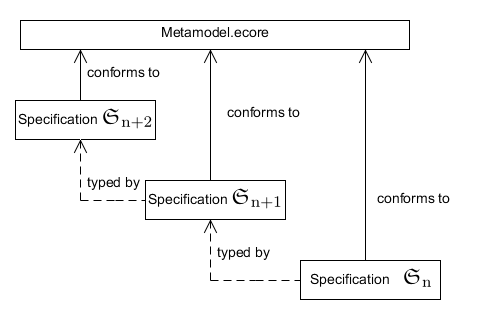
\includegraphics[scale=0.7]{./Figures/metamodelSpecification.png}
	\caption[Specification relationship with core meta-model]
	{Relationship between layers of specification.}
	\label{fig:core_metamodel}
\end{figure}

Figure~\ref{fig:core_metamodel} gives a representation on how specifications
are related and regardless of level of abstraction every specification
$\spec{S}$\textsubscript{1\ldots n} conforms to one common meta-model. For
Henshin we can import this meta-model, \textit{Meatmodel.ecore} that is
provided by DPF. We can use this meta-model in Henshin to define the
content of the transformation rules since every specification
$\spec{S}$\textsubscript{n} conforms to this meta-model. However, other than
consisting of an underlying graph and a set of constraints, a DPF specification
$\spec{S}$\textsubscript{n} is also typed by another
specification$\spec{S}$\textsubscript{n+1}, and this is where it gets
challenging. Because in DPF a specification model $\spec{S}$\textsubscript{n} is
created as an instance from a specification model $\spec{S}$\textsubscript{n+1}.
This is where we have to find a work around for our solution, because we cannot
import an instance model of an Ecore based meta-model into the Henshin model
transformation environment. We can do changes to an instance model by using
Henshin, but the transformation language can only import and utilize models
that conforms to the Ecore meta-model. To solve this for DPF models we expand
transformation rules in Henshin with application conditions. We will look more
closely to how this is done later in this chapter, but what we basically do is
that we restrict the LHS graph to locate matching modeling elements in an
instance model based on the abstract syntax that another instance model
provides. 

%----------------------------------------------------------------------------------------
%	SECTION 2
%----------------------------------------------------------------------------------------

\section{Henshin meta-model}
\label{sec:henshin_meta}

The Henshin transformation language provides a meta-model that is an EMF based
model and uses the Ecore meta-model for typing purposes\cite{Arendt2010}. Since
this model is created based on EMF we know that EMF will generate interfaces and
a factory that we can utilize to implement Henshin transformation rules in Java.
We can specify a pattern graph and a replacement graph for each transformation
rule based on the factory class that Henshin provides. In the following we
will address what elements a transformation rule in Henshin consist of based on
the Henshin meta-model for a transformation rule represented in
figure~\ref{fig:Henshin_metamodel}.
 

\begin{figure}[H]
	\centering
	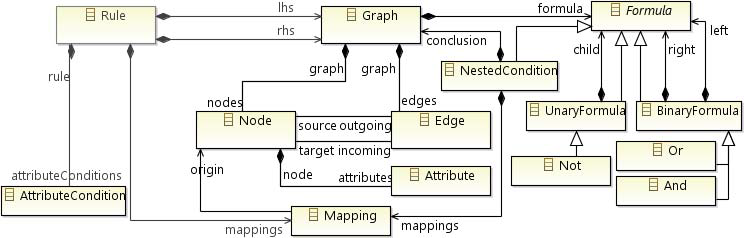
\includegraphics[scale=0.8]{./Figures/Henshin_metamodel.png}
	\caption[Henshin transformation meta-model]
	{Henshin transformation meta-model\cite{Arendt2010}.}
	\label{fig:Henshin_metamodel}
\end{figure}

A \textbf{Rule} in Henshin represents a transformation rule that has a name,
a description and three properties. The first property disables or enables the
transformation rule, while the two other properties lets the user enable or
disable injective matching and the check dangling condition. The rule class
works as the root for all other elements that are represented in 
figure~\ref{fig:Henshin_metamodel}. A new rule defines a left hand side and a
right hand side \textbf{Graph}. The content of the LHS graph represents the
model pattern used to locate matches in an instance graph while the RHS
represents the model pattern that is created. The LHS and RHS graph is formed by
creating nodes and edges. Nodes refers to objects in an instance graph and
edges refer to references between objects. An edge has a source and a target
node, while a node can have a collection of incoming and outgoing edges. The
nodes can also have a set of attributes attached. Nodes, edges and attributes
all have two common properties, and the first one is that they all have a type.
This type is a reference to either an EClass, EReference or EAttribute, that is
all classes of the Ecore meta-model. For example a node that is typed by a
specific EClass will only be matched to objects of this type in an instance
graph. These nodes and edges are represented under a graph and form a pattern.
Together with the LHS and the RHS these patterns is either used to find
matching patterns in a source model or to create the corresponding pattern for
a target model. The second property that these three have in common is that
they have an action type. Action types are predefined stereotypes for Henshin
and specifies how these three Henshin modeling elements of a graph in Henshin
behaves when applying a transformation rule. An action type could specify if a
graph element is part of an application condition, the replacement graph, the
pattern graph or an intersection graph. A\textbf{Mapping} is how
Henshin specifies if nodes are part of this intersection graph, and that is
nodes that are part of both the LHS and the RHS graph. This means that these
objects should be part of the matching pattern, but should not be deleted. A
mapping has two properties, namely an origin and an image. The origin property
refers to a given node, while the image property specify that another node has
a mapping to this node. So far we have a rule that can have two graphs and a
set of mappings. 

A rule can also specify application conditions that determines where a specific
rule could be applied. These application conditions are defined in the
\textbf{Formula} class and is a child of a graph. This formula can either be an
u-nary logical operation, a binary logical operation or a nested condition. The
first logical operation operates on a single operand while the second operates on two
operands, where these operands are represented as a conditional statement that
is either true or false. A rule can be applied to a instance graph if and only
if all application conditions are valid. We can basically have a unlimited
nested formulas in Henshin, since a binary formula can have a right and left
\textbf{Formula}, that can again be of type binary formula. Henshin however is
only concerned with if this formula is valid or invalid when a transformation
rule is applied. A nested condition is required if we want to have nodes that
are part of the LHS graphs or the common graph, that is the intersection of the
LHS and RHS graph. A nested condition provides a graph and a set of mappings to
elements that are part of the LHS or common graph. This graph is child of
a nested condition and contains nodes, edges and attributes that form a
structural pattern that specifies an application condition. We can observe that
a transformation rules can have several number of application conditions. A
binary formula can be of type \textbf{Or} or \textbf{And} and provides the
possibility to nest other binary formulas. If the structure of a binary formula
is the latter, then all the application conditions from both the right and left
formula has to be be valid for a transformation rule to be applied to a
instance graph.

\section{Transform Model Editor}

With the Eclipse Modeling Framework we created an Eclipse plugin where users can
create and modify transformation rules. Figure~\ref{fig:transform_metamodel}
provides the structural data model that we use to generate code for the
implementation of the model and the plugin. The two classes Transform and
Production are the two domain classes that together defines this domain specific
modeling language that lets users create transformation rules. The Transform
class represent the Transform Model Editor and has a source meta-model and a
target meta-model, that corresponds to a source specification and a target
specification. If these two models are the same model, then the model
transformation is an endogenous model transformation and if the models are
different, then we have an exogenous model transformation. We also have the file
location on the storage unit for the source and target meta-model. The rules
represents a collection of the transformation rules. These rules are typed by a
Production and represent one single transformation rule. A transformation
rule has a name and contains a graph that is stored internally for each rule.
This graph contains a pattern of nodes and arrows that the user can edit to
form a LHS graph and a RHS graph. A single Production also has several
collections that contains nodes and arrows. These collections are utilized by
Henshin to generate transformation rules. 

\begin{figure}[H]
	\centering
	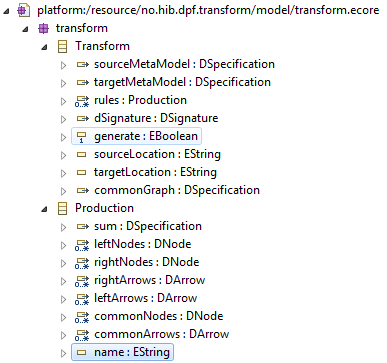
\includegraphics[scale=0.8]{./Figures/transform_metamodel.png}
	\caption[Model for the DPF transformation editor]
	{The domain model to create a DPF model transformation editor.}
	\label{fig:transform_metamodel}
\end{figure}

The user has to invoke the file creation wizard for the Transform Model Editor.
Other than choosing a project folder and a name for this new editor file, the
user has to specify what model is the source meta-model and what model is the
target meta-model. If the user do not specify a target meta-model then the file
creation wizard will interpret this as an endogenous model transformation.

The Transform Model Editor plugin has two editors that users can interact with.
The first is the master editor for the plugin and contains a list of the
transformation rules, where users can create, read, update and delete rules. The
second editor is administrated by the master editor, and each time a new
transformation rule is chosen, a simple version of the DPF editor is opened
with its corresponding transformation rule. This editor is created from the 
Graphical Editing Framework (GEF) and is a graphical editor that includes a
palette. This palette is the same palette that is used in the DPF Editor and
contains modeling elements from the source meta-model and the target meta-model.

\begin{figure}[H]
	\centering
	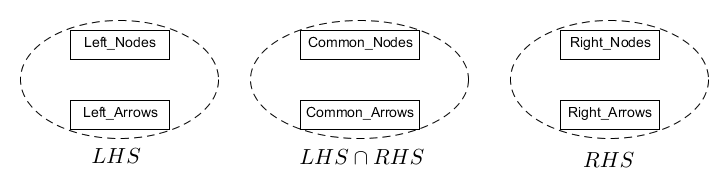
\includegraphics[scale=0.7]{./Figures/left_common_right.png}
	\caption[The three subgraphs for a transformation rule.]
	{Three subgraphs for each transformation rule in the editor.}
	\label{fig:lists_editor}
\end{figure}

These nodes and arrows are used to create the internal graph for each
corresponding rule. For each rule the users can uniquely map nodes and arrows to
three subgraphs represented as lists. Figure~\ref{fig:lists_editor} represents
the left, right and common subgraphs, where each corresponding subgraph
has a list of nodes and arrows. Each subgraph represents a different part of a
transformation rule according to graph transformation. The left subgraph
represents the LHS graph of a rule, while the right subgraph represents the RHS
graph. The common subgraph represents the intersection between the pattern
graph and the replacement graph. It is vital for the model transformation to
work that all the nodes and arrows are mapped to one of these three graphs.
This is entirely up to the user, because the nodes and arrows from the LHS
graph have to be created in such a way that the graph can be matched in an
instance graph.

Now that a list of transformation rules has been specified the user has to
initialise the model transformation environment. This is done through three
steps. 

\begin{enumerate}

\item \textbf{Generate Correspondence Graph.} The first thing the user has to
initialise a graph that contains the correspondence objects. This is important since
Henshin cannot foresee how modeling elements from the source model are related
to modeling elements from the target model. This relation has to be specified
before we can create the Henshin model transformation environment. 

\item \textbf{Generate Henshin Rules.} Before we can use the Henshin model
transformation language we have to provide a module that contains a set of transformation
rules. And to achieve this we have to translate our transformation rules we
create in the editor into Henshin executable rules. 

\item \textbf{Apply Model Transformation.} Now the user has created a
correspondence graph that bind objects from source and target model. Then the
editor generates a Henshin module that contains Henshin executable
transformation rules. We can now apply the transformation rules through
programmatically invoking the Henshin interpreter. 

\end{enumerate}


\section{Generate Correspondence Graph}

The Henshin transformation language refers to modeling elements from a source
specification and a target specification when creating transformation rules. But
we have to define how modeling elements from a source model is translated to a
target model. Henshin is unable to figure out how source modeling elements are
related to target modeling elements unless this is provided explicitly. We can
create a new DPF model that presents all the nodes and arrows from the source
meta-model and target meta-model as nodes.
Figure~\ref{fig:Solution_CorrespondanceObjects} express how we want to implement
this for our model transformation environment.

\begin{figure}[H]
	\centering
	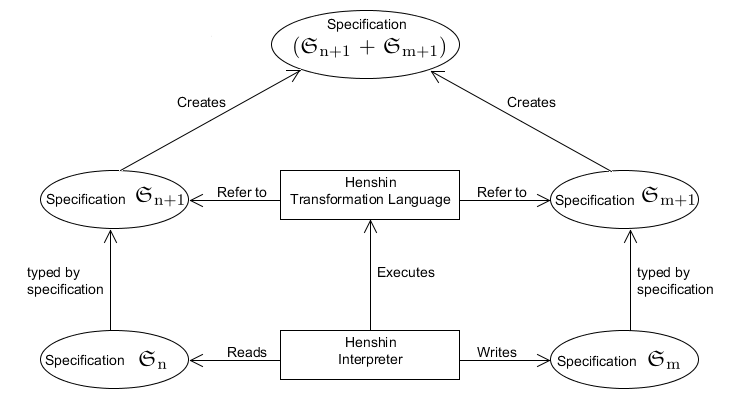
\includegraphics[scale=0.7]{./Figures/TransformationSolution_Correspond.png}
	\caption[Specification for the correspondence objects]
	{The solution expanded with a specification for the correspondence objects.}
	\label{fig:Solution_CorrespondanceObjects}
\end{figure}

Now we have a created a new DPF model contains a list of nodes for all node and
arrow types from the source specification $\spec{S}$\textsubscript{n+1} and
target specification $\spec{S}$\textsubscript{m+1}. We then provide a new
modeling element that is a bridge element between a source and target modeling
element. We can specify an arbitrary number of these elements that binds nodes
and arrows from a source model to nodes and arrows from a target model. This DPF
model specify the correspondence graph between source and target meta-models. We
can now refer to this DPF model when creating Henshin transformation rules to
extract the corresponding objects. We can also do this explicitly when creating
the transformation rules in the Transform Model Editor by modeling a new trace
object that is represents a trace between a source modeling element and a
target modeling element. We use this trace object or the correspondence graph to
determine how we translate a DPF model. We create a trace object that has a
source reference to every matching node and arrow that the transformation engine
can locate and a target reference to the created nodes and arrows. The next
section will address these traceable links in more detail together with how we
generate Henshin transformation rules. 


\section{Generate Henshin Rules}

We utilize the meta-model represented in figure~\ref{fig:Henshin_metamodel} to
create transformation rules in Henshin.  We use the factory that is provided by
EMF for Henshin model transformations to achieve this.
We start with creating the root element that is required for a Henshin model
transformation and import EPackages that is needed to define the content of a
transformation rule. We need to import two models if we want to translate a
specification with Henshin. The first model is the corresponding meta-model for
all specifications and the second model is the meta-model for including
traceable links in Henshin. We will describe the purpose of these traceable
links in more detail in chapter 6.5.1. The transformation language requires
models that define the abstract syntax for an instance model to be able to
specify modeling elements for both the LHS and the RHS of a transformation
rule. We can use meta-elements provided by these two models when defining new
nodes, edges and attributes in Henshin. These types are EClass for nodes,
EReference for edges and EAttribute for attributes. 

For Henshin we create one rule for each production provided by the editor, where
the name of the rule is acquired from the production. Henshin
provides a LHS, a RHS graph and a collection of mappings for each rule. We can
create a graph structure for the LHS and the RHS based on the subgraphs that a
production provides. Modeling elements that form a pattern in the LHS are used
to find a match in a source model, while modeling elements that form a pattern
in the RHS are used to create new elements or replace these elements. Henshin
also include an intersection graph for each rule. This graph is not represented
as a physical graph like the LHS and the RHS are, but is represented as an
underlying graph that is formed from these two graphs. The intersection graph is
represented by having elements in both the LHS and the RHS graph with mappings
that distinguish that these elements are one and the same. Now we have the LHS
graph, the RHS graph and the intersection of these two graphs, which we talked
about in section~\ref{sec:graph_based}. In this section we introduced double
and single pushouts of graphs. Henshin has an arbitrary mixing of these graph
transformation styles.

For each rule we created in the Transform Model Editor we have defined a
pattern, that either corresponds to a left hand side, a right hand side or a
common graph. This pattern consist of nodes and arrows that together form a
graph. For each node and arrow, we create a Henshin node that is either typed
as a Node or as an Arrow. An Arrow has to be represented as a Henshin node since
it is defined in the meta-model for a specification as an EClass. Now we have to
connect Henshin nodes with edges. An edge has three parameters, namely source,
target and reference. In Henshin we create an edge with a source Henshin node
and a target Henshin node. How the reference is typed depends on how the
source and target node refer to each other in the specification meta-model.
Figure~\ref{fig:arrow_node_relate} explains a simple example on how
the relationship between a node and an arrow are handled for a specification.

\begin{figure}[H] 
	\centering
	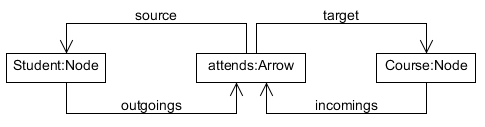
\includegraphics[scale=0.8]{./Figures/arrow_node_relate.png}
	\caption[Relationship between node and arrow in DPF]
	{Example of how nodes and arrows are related for a specification.}
	\label{fig:arrow_node_relate}
\end{figure}

This is a representation on how DPF models relate to one another. We can have an
arrow that has a target and a source node, while every node can have a list of
both incoming and outgoing arrows. So this means that a Node and an Arrow have a
similar relation in DPF models, where source and outgoings references represents
the same relation but are typed differently. It is however easier to coupe with
the arrows when creating transformation rules, since an arrow has an
one-to-one relationship, that means an arrow has one source node and one
target node. How the typing for an edge in Henshin is specified depends on the
Henshin source and target node. These nodes are typed by a corresponding EClass
type from the specification meta-model, that is a Node and an Arrow. An edge in
Henshin can specify a relation between two other Henshin
nodes depending on how references between Node and Arrow are typed. According to
figure~\ref{fig:arrow_node_relate} we have two references between arrow and
node and two references between node and arrow. If the source Henshin node for
an edge is typed by Arrow then the available references are source and target.
On the other side if the source Henshin node is typed by Node then we have a
zero to many relationship in the two references incomings and outgoings. When we
define relationships between two Henshin nodes we use the source and target
reference. This is because this is an one to one relationship between two nodes
and therefore we can always find the source and target node for a given arrow.
This means for every Henshin node that are typed by Arrow we have to specify two
relationships for this Henshin node. This is done by creating two edges in
Henshin, where one refer to source node while the other edge refer to
target node. This is achieved by specifying the Henshin node that is typed by
Arrow as source for both edges and switch between source and target as reference
for each target Henshin node. 

At this moment the pattern on the left hand side and the right hand side graph
are not typed. The pattern conforms to the meta-model for a specification, but
this is the case for all specifications, on every level of meta-modeling. However,
these specification models are typed by another specification, and this is
where we can retrieve the types for every node and arrow. In the specification
meta-model both the Node and Arrow class has a reference type to another Node
and Arrow. Figure~\ref{fig:pac_henshin} represent the LHS for the
Transform Model Editor that we want to generate Henshin rules from. The idea is
to create an application condition for every node and arrow with their
corresponding type node and type arrow. The type nodes and arrows have an
attribute called name and is a string. We can use this attribute to specify a
positive application condition in Henshin. A positive application condition in
Henshin has an action type, require. This means that all application conditions
for Henshin that is typed by this action are required to be valid when searching
through a source model for a transformation rule to be applied. 

\begin{figure}[H] 
	\centering
	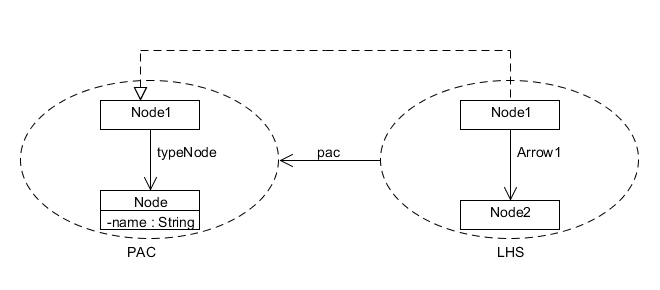
\includegraphics[scale=0.7]{./Figures/PAC_Henshin.png}
	\caption[How we want to handled types for a DPF model]
	{Example on how we want to handled types for a DPF model.}
	\label{fig:pac_henshin}
\end{figure}

This also leads to an important change in our Henshin rules, because we have to
include one more node and edge for every node and arrow. We have to create a new
Henshin node that represent the type node and type arrow. We also have to create
a new Henshin edge that define that this Henshin node is typed by another
Henshin node. This is because when Henshin is locating matches in an instance
graph we want the transformation language to locate matches for nodes or
arrows that are typed by a specific node or arrow. 
Figure~\ref{fig:pac_henshin_condition} explains how we solve this in Henshin.
We have a pattern graph on the right and an application condition graph on the
left. For this rule, we created a pattern graph from a simple graph that the LHS
prov figure~\ref{fig:pac_henshin} the LHS is represented as a simple
directed graph, with an Arrow1 that has a source Node1 and a target Node2. For
this example we focus on the Node1 element.

\begin{figure}[H] 
	\centering
	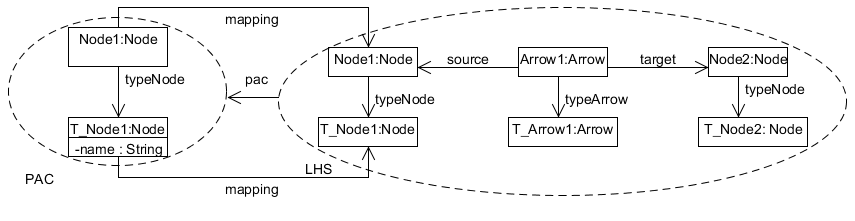
\includegraphics[scale=0.7]{./Figures/PAC_to_Henshin.png}
	\caption[How to handle node types for a rule in Henshin]
	{Defining a transformation rule in Henshin with typing for a
	specification.}
	\label{fig:pac_henshin_condition}
\end{figure}

We discussed in section~\ref{sec:henshin_meta} that an application condition is
represented as a Formula in Henshin, and to solve typing of nodes and arrows in
DPF we need to create this Formula as a nested condition. This is because a
nested condition provides a set of mappings and a graph, where we can define
nodes, edges and attributes. To be able to map Henshin nodes is essential for
creating an application condition. We need to make sure that an application
condition is applied to a corresponding matched modeling element for a source
model. This is achieved by mapping Henshin nodes that are part of the graph in a
nested condition to Henshin nodes that are part of the graph pattern that
is used to locate matches. If we refer back to
figure~\ref{fig:pac_henshin_condition} we can see that the pattern graph has a
Node1 that are typed by a T\textunderscore Node1. We then create a graph for a
nested condition that contains these two nodes and create a mapping from nodes
in the application condition to the nodes in the LHS or intersection graph. It
is important to specify that application conditions can not be defined for the
replacement graph and is not needed either, since the replacement graph is what
we want to translate depending on how many times we can locate a match for the
graph pattern that the LHS provides in an instance graph. Now we need to specify
what an application condition should restrict when searching through matches,
and this is the name attribute of the type element. This application condition
can either be a positive or negative application condition. In this case we want
the name attribute to be a positive application conditions that returns true for
every matching type element located in an instance graph. We can specify
several application conditions for a rule, and it depends on the graph structure
of the searching graph. We define a new application condition for each nodes and
arrows that are part of the LHS graph, since these modeling elements can form a
directed graph and each modeling element is typed by a modeling element from the
source meta-model. All of these application conditions has to be true for a
located match to be a valid match. Now we will look how we also implement
negative application conditions for our model transformation environment with
traceable links. 

\subsection{Traceable links}

As we discussed in chapter 3.2.7 a traceable link works as the footprint when
executing a set of transformation rules. Henshin provides a traceable link
implementation through the Henshin Trace model. This is a simple meta-model for
defining traceable links and can be imported for any Henshin module. The Henshin
Trace model provides a Trace modeling element and provides an unique traceable
link between a source modeling element and target modeling element. The source
and target modeling elements can be any classes that conforms to the Ecore
meta-model. We create a traceable link for every Henshin node we have included
for the LHS graph. The nodes in the LHS graph are the source modeling elements
for a Trace modeling element while nodes in the RHS graph are the target
modeling elements. Now we have an unique link between a matched node from the
LHS graph and a created node for the RHS graph for every time a transformation
rule is applied. These traceable links are represented in the replacement graph
the first time that a connection between two nodes are initialised. This means
that the traceable links are actually translated when a transformation rule is
applied and stored in the translated graph. Next time we want to refer to
a traceable link between modeling elements where a transformation rule has been
applied we have to make sure that the trace object is created both in the LHS
and the RHS with a mapping between them. Because together with a negative
application condition this traceable link will make sure that we only translate
located matches in an source model once. This can be achieved by defining a
negative application condition that forbids Henshin to create a traceable link.
We create a nested condition similar to the previous section, but for this case
we want the application condition only to return true for all matches that does
not contain this graph pattern. This is very convenient when applying a set of
transformation rules, because we have already stated that a traceable link is
created when a transformation rule locates a match in an instance graph. This
means that we create unique traceable links between all nodes in the pattern
graph that is matched in an instance graph and the nodes that we create. One
thing that is worth noticing is that the source and target nodes of a traceable
link has to be typed by the EClass modeling element that Ecore provides. We
can now execute the set of transformation as long as we want and be safe that we
will not execute matching pattern in an instance graph more than once. The
reason that we can make this statement is because when we find a match for the
first time then there exist no traceable link between modeling elements. But
once the transformation engine execute this rule, then a traceable link is
created between the matching nodes on the left side and the corresponding
modeling elements on the right side. And now the transformation engine are
unable to locate this match for a second time because we have restricted the
transformation rule to not include matches that has a traceable link to the
source node that are part of the LHS graph. Now we will describe more in detail
how we apply these transformation rules. 

\section{Apply Model Transformation}

When we have generated all the transformation rules from the Transform Model
Editor to Henshin transformation rules. The Henshin module we generated in the
previous section now contains a set of transformation rules that are specified
in the Henshin Transformation Language, that we described in 
figure~\ref{fig:Simple_Solution} in the first section. Now we have to use the
Henshin Transformation Engine to execute the generated module. We can do this by
explicitly invoking the Henshin interpreter. The interpreter requires a
module, a graph that contains the source model and a Henshin unit before it can be
applied. For our solution we have created a transformation unit that
executes a set of transformation rules in the same order that the Transform
Model Editor provides, and is called a Sequential unit. A transformation unit
in Henshin is an implementation of a rule application control system that we
described in a more general term in section 3.2.3. A transformation unit in
Henshin is an executable part that the transformation engine can interpret and
apply rules accordingly. It is important to specify that a transformation rule
itself in Henshin is a transformation unit, and can therefore be executed by
Henshin's transformation engine. But an Henshin transformation rule does not
provide any control mechanism for it self or other rules when executed.
A transformation rule will therefore only locate one single match if we
invoke the Henshin interpreter on a single rule. This is one reason for why we want to
specify a transformation unit that has some unique properties that a single
transformation rule does not provide. In Henshin transformation units have te
possibility to have other transformation units as subunits.
This means that we have the possibility to create nested transformation units,
and that is what we have done for this solution. The Sequential unit that the
module provides works as the master unit for applying the transformation rules.
For each transformation rule we created in the previous section we define a
Henshin Loop unit. This unit can only contain one single subgraph, and that is
the corresponding transformation rule. The Loop unit is executed for as long as
there are any matching modeling elements in an instance graph and will locate 
matches an unlimited number of times unless we provide any mechanism to stop
the unit. This is where the negative application conditions that we described
in the previous section plays a vital role. Because the negative application
condition specifies that a transformation rule will only be applied unless
there exist no traceable links. The first time the transformation engine
locates a match for a transformation rule it will create a traceable links that
connects the matching modeling elements and the created modeling elements. Now
the next time this specific match is located the application condition will not
be valid since now there are traceable links that has references to modeling
elements in the source model. We can now apply these repeatable units for all
transformation rules as long as the input graph does not contain a traceable
link for a matched modeling element. 

For all matches found in a source model we do some changes depending on how the
RHS graph is specified. These changes can be found as new DPF modeling elements
after a model transformation for the input graph. We can then extract these
changes and create a new specification that forms the target model. We have to
make sure that the new specification is typed by a corresponding specification,
that is the target meta-model. We can then make sure that the translated
nodes and arrows are assigned with the corresponding type. Since we translated
matches that have one matching node and one matching type node into target
modeling elements that also have a node and a type node.




